\section{Specification}
Formal verification requires both a system model and a specification. This means that the project stakeholders must provide an exact definition of the desirable system properties. Furthermore, it is often the case that such properties are expressed as occurring only under certain conditions. For convenience we provide the symbols used to describe the vehicle specification in Table \ref{table:vehiclespec}.
\begin{table}[h]
	\centering
	\caption{Symbols for Specifications}
	\label{table:vehiclespec}
	\begin{tabular}{|c|c|c|}
		\hline
		\multicolumn{3}{|c|}{Symbol List} \\ \hline
		Symbol & Units & Description \\ \hline
		$k$ & - & Search Depth \\ \hline
		$\phi$ & - & Ego Vehicle Spec \\ \hline
		$\xi$ & - & Environment Spec \\ \hline
		$LC$ & Boolean & Lane Change Request \\ \hline
		$LO$ & Boolean & Lane Occupied \\ \hline
		$v_{ego}$ & m/s & Velocity of Ego Vehicle \\ \hline
		$s_{x_{ego}}$ & m & Position of Ego Vehicle, x \\ \hline
		$s_{y_{ego}}$ & m & Position of Ego Vehicle, y \\ \hline
		$v_{limit}$ & m/s & Speed Limit \\ \hline
		$s_{x_{ref}}$ & m & Centerline Reference, x \\ \hline
		$s_{y_{ref}}$ & m & Centerline Reference, y \\ \hline
		$w(s_{x_{ref}},s_{y_{ref}})$ & m & Lane Width \\ \hline
		$B$ & m & Buffer\\ \hline
		$r$ & m & Collision Radius \\ \hline
		$t$ & s & Current Timestep \\ \hline
		$t_{max}$ & s & Max Timestep \\ \hline
		$\Box$ & - & Always \\ \hline
		$\to$ & - & Implies \\ \hline
		$\neg$ & - & Not \\ \hline
		$ \wedge$ & - & And \\ \hline
		$ \vee$ & - & Or \\ \hline
	\end{tabular}	
\end{table}
\label{sec:exp specification}

\pagebreak
 An example specification follows: the ego vehicle should drive in the selected lane at the speed limit \emph{unless} a stop sign is encountered. We note that the traffic laws of a given region provide a partial, but informal definition of many of the high level specifications which the ego vehicle should adhere to. 

\subsection{Ego Vehicle Specifcation}
The specification for the ego vehicle has two components: safety properties and liveness properties. A specification for the ego vehicle in the case study follows:
\begin{itemize}
	\item The ego vehicle travels at a velocity less than or equal to the speed limit
	\begin{equation}
		\Box \left(v_{ego} \leq v_{limit}\right)
	\end{equation}
	\item The ego vehicle does not drive backwards
	\begin{equation}
		\Box \left( v_{ego} \geq 0 \right)
	\end{equation}
	\item The ego vehicle does not collide with any of the $n$ other objects in the environment
	\begin{gather}
		\Box \left( \sqrt{(s_{x_{ego}} - s_{x_{env_i}})^2 + (s_{y_{ego}}- s_{y_{env_i}})^2 }  \geq r \right) \notag \\ \forall i = 1...n 
	\end{gather}
	\item If a timed lane change request is invoked, the ego vehicle completes the lane change on time.
	\begin{equation}
		\Box \left( LC \to \left(s_{y_{ego}} > w\right) \wedge \left(t \leq t_{max}\right)\right)
	\end{equation}
\end{itemize}

\subsection{Environment Specification}
The other vehicles operating within a scenario present both an interesting challenge and a primary motivation for formal verification. It is clear that it is impossible to know the intentions of the agents operating such vehicles; their execution represents a significant source of non-determinism. In fact, a more complex model of such agents which includes details such as steering angle or tire friction will not enable less conservative results, for it is the control input not the plant that remains the largest unknown. Thus, we conclude that:
{\it for verifying the autonomous agent, only the perceptible behavior of other agents is important, not their internal structure.}

Still it remains clear that {\it the behavior of other agents must be part of the scenario description.} As such we present a safety case which assumes that other agents will follow a certain minimal set of driving rules. For brevity we will reference the following specification as $\xi$ in the case studies.% as specified in \cite{Althoff2014} which is a subset of the Vienna Convention on Road Traffic \cite{Europe.TransportDivision2007}:

\begin{itemize}
	\item Acceleration ceases when some maximum velocity is reached.
	\begin{equation}
		\Box \left( v_{env} \geq v_{max} \to a = 0 \right)
	\end{equation}
	\item Other agents must drive in the proper direction according to their lane.
	\begin{equation}
		\Box \left( v_{env} \geq 0 \right)
	\end{equation}
	\item The accelerations of other agents are within those rates achievable by maximum engine power
	\begin{equation}
		\Box \left( a_{env} \leq a_{max}\right)
	\end{equation}
	\item Other agents maintain their lanes unless explicitly specified not to.
	\begin{equation}
		\Box \left( \neg LC \to \left( y_{min} \leq s_{y_{env}} \right) \wedge \left( y_{max} \geq s_{y_{env}} \right) \right)
	\end{equation}
	\item Lane changes by other agents are only permitted if the alternate lane is unoccupied or unless a degenerate scenario is being modeled.
	\begin{equation}
		\Box \left( LO \to \neg LC \right)
	\end{equation}
	
\end{itemize}

\section{APEX internals and theory}
\label{sec:apex internals}

APEX maintains an internal representation of the scenario as a \emph{hybrid system}.
The components of this hybrid system are:
\begin{itemize}
	\item The behavioral planners of all vehicles involved, $\Bc_1,\ldots,\Bc_m$.
	Fig. \ref{fig:beh planner} shows the behavioral planner we used in the case study for a lane change.
	A behavioral planner is a finite state system. 
	We will refer to each state of a behavioral planner as a \emph{mode}.	
	\item For every vehicle, the continuous dynamics involved in each of the modes of its behavioral planner.
	%	These dynamics govern the evolution of the continuous state $x_i \in \Re^N$ which includes position, velocity, etc, of the vehicle.
	In general, different modes may require different dynamics: e.g. a Collision Avoidance mode which is invoked when a collision is imminent requires more stability control than a turn at a low speed.
	The continuous dynamics are given in terms of Ordinary Differential Equations (ODEs) $\dot{x}_i = f_i(x_i)$, 
	where $x_i \in R^n$ is the continuous state of the $i^{th}$ agent.
	%
	\item For each vehicle, transition conditions between the modes of the behavioral planner $\Bc_i$ are expressed in terms of the state vector $x_i$.
	The planner transitions between two modes $q$ and $q'$ only if a \emph{guard condition} $G_{q,q'}$ is satisfied.
	In general, the guard condition for $\Bc_i$ is expressed as a set in the state space of \emph{all the agents}, since transitions will occur based on, for example, how close two vehicles are to each other.
	Specifically, let $x = (x_1,\ldots,x_n)$ combine the states $x_i$ of the individual vehicles.
	So $x \in R^{n\cdot m}$.
	Then there's a transition between two states $q$ and $q'$ of $\Bc_i$ only if $x \in G_{qq'} \subset R^{n\cdot m}$.
	For example, there's a LF-to-LC transition only if the two cars are closer than $10m$ and the following car is faster than the leading car.
	In this case $G_{LF,LC} = \{x \;|\; ||x_1 - x_2|| \leq 10 \land v_2 > v_1\}$.
\end{itemize}
Together, these make up a hybrid system, so-called because it combines discrete dynamics in the behavioral planner with continuous dynamics in each mode.
We will refer to the $n$ hybrid systems of the $n$ agents in the scenario as $H_1,\ldots,H_m$.
The \emph{state of the scenario} $x$ is simply $x = (x_1,\ldots,x_n)$.

APEX does not keep an internal representation of the motion planner. 
Rather, as explained in earlier sections, APEX issues calls to the motion planner in the course of the verification, and obtains a trajectory from it.

APEX also needs to maintain a description of the scenario specification.
This specification is provided by the user and can be any formula in first-order logic over the set of modes and states of all agents. 
See the \emph{Case Study}.% \ref{sec:specifications}.
For example the following is a possible specification:
\[Mode_1 = LC \to |\dot{\psi}| \leq b \]

The following sections describe how APEX verifies a property of the scenario using this internal representation.

\subsection{Execution tree and formal model}
\label{sec:execution tree}
Let $\Bc$ be a behavioral planner of a given vehicle.
%(For simplicity of description we assume the other vehicles have the same behavioral planner, though in general this need not be the case).
The formal model of the behavioral planner is a finite transition system $\Bc = (Q,q_0, \Sigma, \rightarrow)$ where $Q$ is the finite set of modes, $q_0$ is the initial mode, $\Sigma$ is a set of output labels, and $\rightarrow \subset Q\times \Sigma \times Q$ is the labeled transition relation of the system.
We write $q \trans{\sigma}q'$ for $(q,\sigma,q') \in \trans{}$.
Fig. \ref{fig:beh planner} shows the behavioral planner that is used by APEX by default for modeling a lane change controller.
It can be described as $\Bc = (\{LC, LF\}, LF, R^n, \{(LF,LF), (LF,LC), (LC,LF)\})$.
In mode LF, the vehicle's goal is to follow the current lane.
In mode LC, the vehicle's goal is to change lanes.
In general, a mode represents a decision by the controller, a \emph{behavior} that the vehicle should follow.
With every transition between modes, the behavioral planner outputs a vector $x_B$ in $R^n$: this is the destination that the vehicle must reach.
The planner transitions between modes when certain \emph{guard conditions} are satisfied.

The behavioral planner advances in discrete time.
The discrete time advances, for example, with every update of the vehicle's sensors.
Thus $\Bc$ makes a decision on what to do everytime its information about the environment is updated.
The planner may decide to maintain the current decision, i.e., stay in the same mode, if that mode has a self-loop.
Mode $LF$ has a self-loop in Fig. \ref{fig:beh planner}.
Let $\Delta t >0$ be the update period.
Since every scenario is time-limited, and every transition takes fixed non-zero time $\Delta t$, there is a natural limit $D$ on the number of decisions, or transitions, that can be taken in any given scenario.

In the first step of the verification process, APEX builds an execution tree: the root of the tree is the initial mode $q_0$, and every branch of the tree represents one possible sequence of decisions, i.e. one possible execution of $\Bc$.
See Fig. \ref{fig:extree} for the execution tree of the behavioral planner of Fig. \ref{fig:beh planner}.
Since the number of transitions is bounded by $D$ in a given scenario, this tree has a depth at most $D$.

With the execution tree built, APEX must next verify that the sequence of decisions taken by the behavioral planner can be implemented by the low-level controllers.
E.g., let $(LF,LF,LC)$ be a sequence of decisions of depth 3.
In every occurrence of LF, APEX must check that the vehicle can indeed follow the lane, and in every occurrence of LC, APEX must verify that the vehicle can indeed change lanes.
In the next section, we define what it means to `follow the lane' and 'change lanes' via the motion planner.
%At every discrete time step, $\Bc$ either stays in LF, or transitions to LC, depending on whether the state $x$ of the scenario satisfies the guard set $G$ for the LF-to-LC transition.
%Note that the transition of $\Bc_1$ to LC depends on the states of other cars, not just the state $x_1$ of the ego vehicle.
%Hence, we need to consider whether $x=(x_1,\ldots,x_n)$ is in the guard set or not.

%Before proceeding, we give the rest of the formal model of the scenario in APEX.
%In addition to the mode, each vehicle is also described by its continuous state $x \in R^n$, which contains states such as position, velocity, pose, yaw rate, steering angle, etc.
%Thus the state of the vehicle is given by the pair $(q,x) \equiv h \in Q \times R^n$. 
%At time 0 of the scenario, the initial mode is $q_0$ and the initial state is $x(0) \in X_0 \subset R^n$.
%When the behavioral planner is in mode $q$, the continuous state evolves according to the mode-specific ODE $\dot{x} = f_q(x)$.
%The ODE is mode-specific since in general, depending on the current behavior of the vehicle, different dynamic forces are applied, or with different parameters.
%E.g. stability control is activated in more aggressive maneuvers.

%The decision to switch modes is made depending on the current state $x$. 
%E.g., if two vehicles are closer than some distance, the trailing vehicle will decide to change lanes.
%We may re-express this in terms of guard \emph{sets}:
%the behavioral planner $\Bc_2$ of the trailing vehicle will transition $LF \trans{x_B} LC$ if their states $x_1$, $x_2$ are in the set $\{(x_1,x_2) \;|\; ||(s_{x,1},s_{y,1}) - (s_{x,2},s_{y,2})|| \leq \varepsilon \}$.
%This behavior is formalized by the guard conditions on the transitions of the behavioral planner.
%If we let $x_i$ in $\in R^n$ denote the state of the $i^{th}$ vehicle in the scenario, $i=1,\ldots,m$, 
%then we define $x = (x_1,\ldots,x_m) \in R^{nm}$ to be the state of the scenario.
%Then in the behavioral planner $\Bc_i$, the transition $q_i \trans{\sigma} q_i'$ is taken when $x \in G_{q_iq_i'} \subset R^{nm}$.
%$ G_{q_iq_i'}$ is referred to as a guard set.
%
%When the behavioral planner $\Bc_i$ of the $i^{th}$ vehicle is in mode $q_i$, then $x$ is governed by 
%$\dot{x} = f_q(x) \in R^{n\cdot m}$, where $q = (q_1,\ldots,q_m) \in Q_1 \times \ldots \times Q_m := Q$ and 
%$f(x) = (f_{q_1}(x_1), \ldots, f_{q_m}(x_m))$.
%We may similarly define a composite initial state for the scenario: $q_0 := (q_{0,1},\ldots,q_{0,m})$, and a composite label set $\Sigma = \Sigma_1 \times \ldots \times \Sigma_m$.
%When $\Bc_i$ transitions $q_i \trans{\sigma_i}q_i'$, we consider that the composite system $(\Bc_1,\ldots,\Bc_m)$ transitions $q \trans{\sigma}q'$ where $q$, $q'$ and $\sigma$ are defined in the natural manner.
%
%The composite system $H = (Q,q_0,\Sigma,\trans{}_H,\{f_q\}_{q\in Q}, \{G_{qq'}\}_{(q,*,q') \in \trans{}})$ is a \emph{hybrid system}: it has discrete transitions in its behavioral planner, and continuous evolutions in its continuous states.


\subsection{Calling the motion planner}
\label{sec:calling motion planner}

%\begin{figure}[t]
%	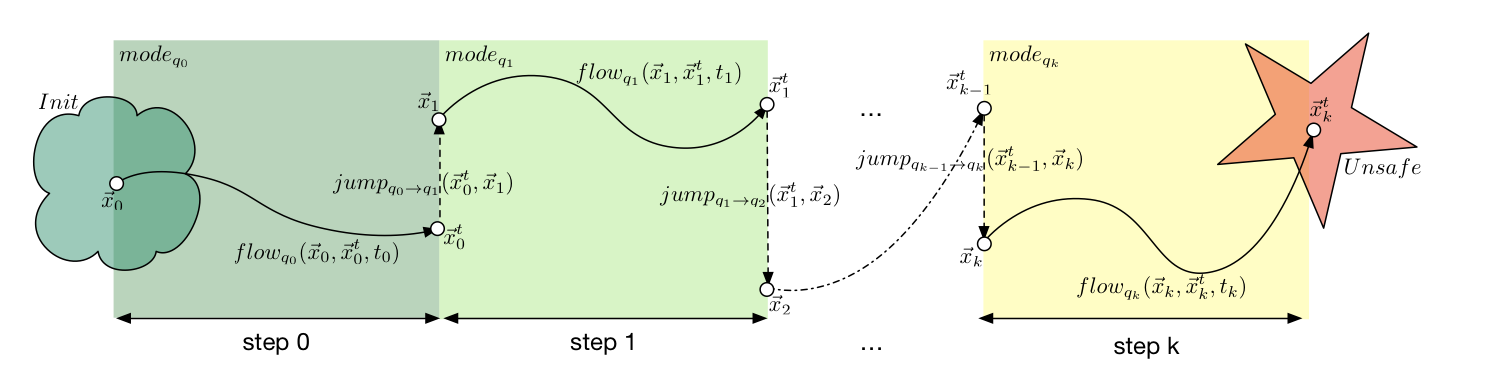
\includegraphics[width=\columnwidth]{figures/unsafe}
%	\caption{The bounded reachability problem in dReach \cite{KongGCC15}}
%	\vspace{-20pt}
%	\label{fig:unsafe}
%\end{figure}

After building the execution tree, APEX starts executing every branch, starting at the root, which is the initial mode $q_0$.
The initial set of continuous states is $X_0$.
A transition is taken if the initial set intersects its guard.
Since $X_0$ may intersect more than one guard, then more than one transition are possible. 
APEX explores all transitions (all branches) in the execution tree.
In each mode APEX enters, $\Bc$ will output a destination $x_B$.
Formally, $x_B$ is a scenario state, but in what remains, it is simpler to think of it as the position that the ego vehicle must reach.

APEX then calls the motion planner to obtain the trajectory that the vehicle will follow.
%See Fig. \ref{fig:apex_internals}.
Since the current state is only known as a set $X_A$, APEX sets the starting point of the trajectory to be the center $x_A$ of $X_A$.
The motion planner then returns a trajectory starting at $x_A$ and ending in a neighborhood of $x_B$.
The neighborhood shape and size are known to APEX and are part of the motion planner's description.
Let that neighborhood be $X_B$. Note that APEX does not place any restrictions on the motion planner's operation and calls it as a black box.
Therefore, the actual motion planner that is used on the real car can be used in the verification of the system.
In this way the verification results are directly applicable to the actual deployed software.

\subsection{Verifying each trajectory}
\label{sec:verif each traj}
Once a trajectory is generated connecting $x_A \in X_A$ to the neighborhood $X_B$ of $x_B$, it remains to verify that the ego vehicle will always reach $X_B$ within a specified amount of time $T$, regardless of where it starts in $X_A$.
To verify that the specification is satisfied, APEX builds a \emph{reachability problem}.
This reachability problem is characterized by the following:
\begin{itemize}
	\item The system: in this case, the system consists of the scenario hybrid system.
	\item The target set: this is the set that the system should reach. 
	In this case the state of the ego vehicle $x_1$ should reach $X_B$, and there are no target sets for the other agents. 
	\item The unsafe set: this is the set that the scenario hybrid system must \emph{not} reach at any point in time.
	In this case, the ego vehicle must not get closer than $d_{min}$ to any other agent in the scenario.
	\item A time bound: the target set must be reached within a certain amount of time $T$.
\end{itemize}

We call the above a bounded reachability problem. %- see Fig. \ref{fig:unsafe}.
To solve this problem, APEX passes it to dReach \cite{KongGCC15}, a reachability analysis tool for nonlinear hybrid systems.
dReach answers the question: is there a trajectory of the vehicle starting in $X_A$ that will violate the constraints? (e.g. will not reach the target set $X_B$ or will get too close to another vehicle).
dReach returns one of two answers.
If the answer dReach returns is SAFE, then it is \emph{guaranteed} that \emph{no} behavior of the ego vehicle will violate the constraints.
It should be stressed that this is a mathematical guarantee: no amount of simulation in this case will reveal a violation, because dReach guarantees that no such violation exists.
If dReach answers $\delta$-UNSAFE, then this means that there exists a behavior of the ego vehicle which, when perturbed by an amount $\delta >0$, violates the constraints.
See Fig. \ref{fig:reachability}.
The parameter $\delta$ can be set by the user.
It suffices to choose $\delta$ small enough so $\delta$-SAT means the system is not robust since a small perturbation of size $\delta$ could cause it to violate the constraints.

%\subsubsection{Hybrid Systems}
%In this section, we define a hybrid system, a formalism for describing mixed discrete-continuous systems. The tuple $\mathcal{H}$ represents a hybrid system:
%\begin{equation}
%\mathcal{H} = \left[ \mathcal{X},\mathcal{Q},\mathcal{X}_{init},\mathcal{X}_{inv},\mathcal{F}(\mathcal{P}),T \right]
%\end{equation} 
%where $\mathcal{X}$ represents the continuous states, $\mathcal{Q}$ denotes the discrete modes, $\mathcal{X}_{init} \in \mathcal{R}_{\mathcal{X}}$ specifies the initial condition space, $\mathcal{F}(\mathcal{P})$ captures the flows parameterized by a vector $\mathcal{P} \in \mathcal{R}_{P}$, $\mathcal{X}_{inv}$ identifies invariants mapping modes to flows, and $T$ relates the transitions between modes. A measurable output $y = \phi (t;\mathcal{X}_{init})$ is a vector which defines an observable state of the system, with $\phi(t,\mathcal{X}_{init})$ describing the measurement at time $t \in [0, t_{\max}]$, having evolved from initial condition $\mathcal{X}_{init}$. 

%The dReach approach utilizes the framework of $\delta$-complete decision procedures that aims to solve first-order logic formulas with arbitrary computable real  functions (\cite{gao2013satisfiability}). 
%The dReach tool can be employed to prove safety properties of hybrid systems over finite time by identifying safe and unsafe regions of the state space and defining a corresponding $\delta$-decision problem. 
%Following \cite{gao2013satisfiability}, we consider the $\delta$-$decision$ problem 
%
%\begin{equation}
%\label{eq:deltadecision}
%\begin{split}
%\exists x_0 \in X_0 \wedge \exists t \in [0,t_{max}] \wedge \exists y \in \mathcal{R}_{unsafe}\\ \mbox{s.t.}
%|x_0| \leq \delta_1 \wedge | y-\phi(t;x_0)| \leq \delta_2
%\end{split}
%\end{equation}
%
%where $\delta_i$ is a numerical error bound specified by an arbitrary rational number \cite{ko1991complexity}.
%
